\documentclass[11pt,a4paper]{article}
\usepackage{tikz}
\usetikzlibrary{arrows.meta,positioning}
\usepackage{tabularx}
\usepackage{amsmath,amssymb,amsthm}
\usepackage{geometry}
\geometry{margin=1in}
\usepackage{hyperref}
\usepackage{graphicx}
\usepackage{setspace}
\onehalfspacing

\title{\textbf{Paper D-13: Population Genetics:\\ A Constraint-Driven Flux Dynamics (CDFD) Perspective}}
\author{Steve Bico Mujjabi, MD\\
\small Independent Researcher\\
\small Founder, Vura Labs\\
\small Kampala, Uganda\\
\small ORCID: 0009-0001-0556-5516}
\date{August 2026}

\begin{document}
\maketitle

% BEGIN SHARED-METHODS POINTER
\noindent\textit{Shared Part IV notation and evidence boundaries are defined in \path{PART_IV_METHODS_AND_CLAIM_BOUNDARY.md}. This paper states only its local observables, comparison, and failure conditions.}
% END SHARED-METHODS POINTER


\begin{abstract}
This paper develops a falsifiable CDFD/AFL model of Population Genetics. It maps mutation, migration, selection, recombination, and reproduction to driving flux $\Phi$, population size, connectivity, resources, drift, and reproductive limits to active constraint $C$, recombination, plasticity, dispersal, mate choice, and adaptation to responsiveness $S$, and allele frequencies, bottlenecks, linkage, environment, and selection history to structural memory $M_s$. The target outcome is diversity, adaptation, fixation, and extinction risk, tested against genomes, pedigrees, experimental evolution, demography, and environmental records. The paper treats universality as a shared model architecture rather than an assertion that unlike systems have the same material mechanism. It states the negative result that would make the mapping unnecessary and places the domain claim inside the cumulative CDFD programme and its reproducible runtime boundary.
\end{abstract}

\section{Introduction}

Evolution is the algorithm by which life explores morphological and functional space. Mutations introduce random variations, gene flow mixes them across geography, and natural selection eliminates variants that are ill-suited to the environment.

In CDFD, this process is formally comparable at the declared-variable level to fluid dynamics. The genome of a population is a fluid network of information passing through time. The environment acts as a restrictive channel that shapes and squeezes this flow.

\section{The Gene Pool as an Adaptive Surface}
We track the evolutionary stability of a species via the Adaptive Operating Ratio:
\begin{equation}
    \Psi_s = \left( \frac{\Phi}{C} \right) \cdot S \cdot M_s
\end{equation}

In the context of population genetics:
\begin{itemize}
    \item \textbf{Flux ($\Phi$)}: The rate of genetic variation introduced by mutation, recombination, and immigration (gene flow). This is the raw informational throughput of the species.
    \item \textbf{Constraint ($C$)}: Natural selection and environmental pressure (predators, climate, resource scarcity). Selection acts as a filter, removing non-viable informational flow.
    \item \textbf{Responsiveness ($S$)}: The genetic diversity and phenotypic plasticity of the population. A highly diverse population can easily flex to meet changing constraints.
    \item \textbf{Memory ($M_s$)}: Genetic fixation and canalization. As a trait becomes heavily selected for, it becomes fixed in the genome. The species "remembers" successful past adaptations, severely restricting future morphological deviations (high $M_s$).
\end{itemize}

\subsection{Extinction vs. Speciation}
A well-adapted species in a stable environment operates at $\Psi_s \approx 1$. The genetic flux ($\Phi$) perfectly matches the environmental constraints ($C$), and the genetic memory ($M_s$) maintains the optimal phenotype.

If the environment suddenly changes (e.g., rapid climate change), the constraint $C$ spikes violently. If the species has low diversity ($S$ is low) and its genome is heavily canalized ($M_s$ is locked), it cannot adapt. The ratio plummets to $\Psi_s \ll 1$. The flow of genes through time ceases entirely---this is \textbf{Extinction}.

Conversely, consider a population spread across a vast area that is suddenly divided by a mountain range. The gene flow ($\Phi$) between the two groups drops to zero. Isolated, each group faces unique local constraints ($C$). To restore $\Psi_s \approx 1$ locally, the responsiveness ($S$) of each group explores different mutational pathways. Over time, their genetic memories ($M_s$) lock into incompatible configurations. The singular adaptive surface has bifurcated into two distinct species. This is \textbf{Speciation}, a direct topological consequence of severing the flux network.



\section{Measurement Layer}

% BEGIN PART IV MAJOR CROSS-DOMAIN UPGRADE
\section{Cross-Domain Model Upgrade: Mechanism, Scale, and Tests}

\subsection{Observable Translation}

The paper-specific translation begins with an observable chain rather than a
verbal analogy. For Population Genetics, the proposed drive is mutation, migration, selection, recombination, and reproduction.
The active limitation is population size, connectivity, resources, drift, and reproductive limits. Responsiveness is carried by
recombination, plasticity, dispersal, mate choice, and adaptation, while retained state is represented by
allele frequencies, bottlenecks, linkage, environment, and selection history. The outcome to explain is diversity, adaptation, fixation, and extinction risk.

\begin{table}[htbp]
\centering
\small
\caption{Operational CDFD/AFL map for Paper D-13.}
\begin{tabularx}{\textwidth}{|l|X|X|}
\hline
\textbf{Term} & \textbf{Paper-specific observable meaning} & \textbf{Measurement question} \\
\hline
$\Phi$ & mutation, migration, selection, recombination, and reproduction & What rate, load, gradient, or demand enters the focal system? \\
\hline
$C$ & population size, connectivity, resources, drift, and reproductive limits & Which measured bottleneck limits transfer, function, or recovery? \\
\hline
$S$ & recombination, plasticity, dispersal, mate choice, and adaptation & Which process changes effective capacity or reroutes the load? \\
\hline
$M_s$ & allele frequencies, bottlenecks, linkage, environment, and selection history & Which retained state makes equal present loads produce different futures? \\
\hline
$Y$ & diversity, adaptation, fixation, and extinction risk & Which outcome is predicted out of sample, with uncertainty? \\
\hline
\end{tabularx}
\end{table}

\begin{figure}[htbp]
\centering
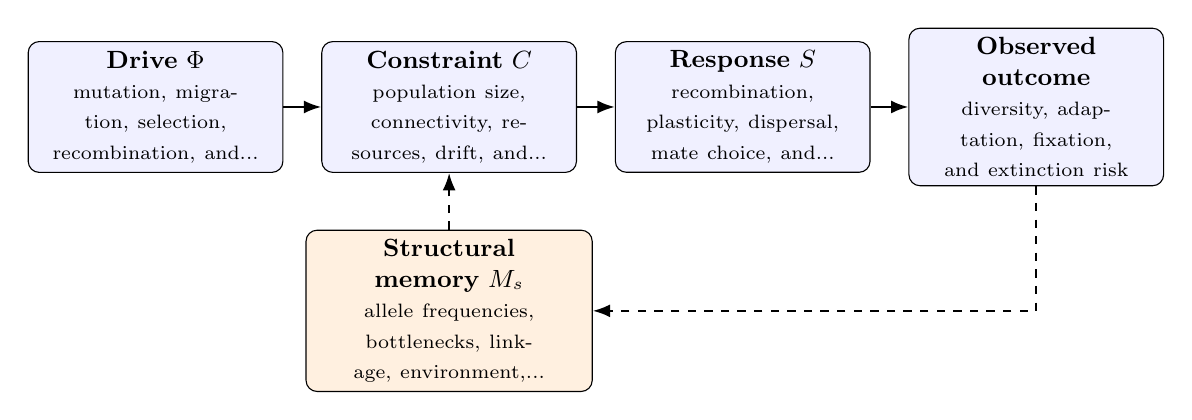
\begin{tikzpicture}[
    node distance=0.48cm,
    every node/.style={font=\small},
    box/.style={draw, rounded corners, align=center, minimum height=1.45cm, text width=3.0cm, fill=blue!6},
    memory/.style={draw, rounded corners, align=center, minimum height=1.25cm, text width=3.4cm, fill=orange!12},
    flow/.style={-{Latex[length=2.2mm]}, thick},
    feedback/.style={-{Latex[length=2.2mm]}, thick, dashed}
]
\node[box] (drive) {\textbf{Drive $\Phi$}\\\scriptsize mutation, migration, selection, recombination, and...};
\node[box, right=of drive] (constraint) {\textbf{Constraint $C$}\\\scriptsize population size, connectivity, resources, drift, and...};
\node[box, right=of constraint] (response) {\textbf{Response $S$}\\\scriptsize recombination, plasticity, dispersal, mate choice, and...};
\node[box, right=of response] (outcome) {\textbf{Observed outcome}\\\scriptsize diversity, adaptation, fixation, and extinction risk};
\node[memory, below=0.72cm of constraint] (memory) {\textbf{Structural memory $M_s$}\\\scriptsize allele frequencies, bottlenecks, linkage, environment,...};
\draw[flow] (drive) -- (constraint);
\draw[flow] (constraint) -- (response);
\draw[flow] (response) -- (outcome);
\draw[feedback] (outcome.south) |- (memory.east);
\draw[feedback] (memory.north) -- (constraint.south);
\end{tikzpicture}
\caption{Paper D-13 observable CDFD/AFL architecture for Population Genetics. Solid arrows give the proposed forward chain; dashed arrows make history-dependent feedback explicit.}
\label{fig:d13-architecture}
\end{figure}

\subsection{Paper-Specific Causal Hypothesis}

For this paper, the hypothesized causal sequence is specific. A change in
mutation, migration, selection, recombination, and reproduction arrives faster than recombination, plasticity, dispersal, mate choice, and adaptation can compensate.
This raises or redistributes population size, connectivity, resources, drift, and reproductive limits. If the load persists,
the retained state encoded by allele frequencies, bottlenecks, linkage, environment, and selection history changes the next response, so a later event of equal
magnitude can produce a different trajectory in diversity, adaptation, fixation, and extinction risk. The
scientific task is to estimate that sequence against the best ordinary model of
the domain, not merely to redescribe the outcome after it occurs.

\subsection{Cross-Scale Translation Without Mechanistic Erasure}

For the domain applications family, the cross-domain translation is a disciplined test across systems with very different material mechanisms. A valid mapping preserves the baseline science of the domain, declares the scale of every variable, and earns its place through a discriminating prediction rather than resemblance alone. \cite{Holling1973,Turing1952,Shannon1948,BakTangWiesenfeld1987}
The required scale declaration for this paper is generations to geological time; loci to metapopulations. At short
scales, the key question is whether the incoming drive is transmitted,
buffered, or diverted. At intermediate scales, response changes effective
capacity and network exposure. At long scales, retained structure can alter the
state space itself. A result is genuinely cross-scale only when the aggregation
rule is stated and the same conclusion is not an artifact of averaging.

\subsection{Evidence Ladder and Discriminating Tests}

\begin{table}[htbp]
\centering
\small
\caption{Evidence ladder for Paper D-13. Each rung can fail independently.}
\begin{tabularx}{\textwidth}{|p{0.17\textwidth}|X|X|}
\hline
\textbf{Test} & \textbf{Design} & \textbf{Discriminating result} \\
\hline
Proxy audit & Measure genomes, pedigrees, experimental evolution, demography, and environmental records and preregister how each record maps to $\Phi$, $C$, $S$, $M_s$, and $Y$. & The mapping fails if proxies are non-identifiable, circular, or change meaning across cases. \\
\hline
Load ramp & Apply or observe a selection or migration shift across populations with different histories while estimating the dominant constraint and response time. & A threshold claim requires a reproducible nonlinear change and uncertainty bounds, not a visually chosen breakpoint. \\
\hline
Recovery and memory & Match present load across units with different histories, then compare recovery paths. & The memory claim requires history-dependent divergence after current conditions are controlled. \\
\hline
Model comparison & Compare the baseline domain model with and without the CDFD/AFL state variables using held-out data. & The paper's stated falsifier is: explicit memory and constraint variables do not improve evolutionary prediction. \\
\hline
\end{tabularx}
\end{table}

\subsection{Research Programme and Boundary Conditions}

The immediate research programme has four steps. First, construct a documented
dataset from genomes, pedigrees, experimental evolution, demography, and environmental records and retain raw units before normalization.
Second, fit a baseline domain model and report its calibration and out-of-sample
error. Third, add the smallest identifiable CDFD/AFL state extension and test
whether it improves prediction of diversity, adaptation, fixation, and extinction risk. Fourth, repeat the
analysis across the declared scale range and publish negative cases as part of
the cross-domain translation audit.

% END PART IV MAJOR CROSS-DOMAIN UPGRADE

\section{Conclusion}
The mathematics of evolution are the mathematics of constrained flow. By applying CDFD to population genetics, we eliminate the false dichotomy between biology and physics. The gene pool flows, adapts, and breaks around environmental constraints in a comparable but materially distinct manner that a river carves a canyon or a language splinters into dialects.
\section*{Conflict of Interest} The author declares no conflict of interest.
\section*{Data Availability}
Part-specific runtime diagnostics are under each Part's \path{outputs/} directory.

Release-wide code: \path{Part_E_Synthesis/supplementary/}.

Generated summaries: \path{Part_E_Synthesis/outputs/}.

Figures: \path{Part_E_Synthesis/figures/}.


\section{Reference Layer}
\bibliographystyle{plain}
\bibliography{universal_afl_references}
\end{document}
